\chapter{\label{ch:chargeid}Charge Identification with Convolutional Neural 
Networks} 

\minitoc

A major problem faced by the next generation of neutrino experiments
is the correct categorisation of particle interactions within the detector.
Typically identifying the underlying type of a neutrino interaction involves
determining the lepton content of the final state particles; as such it is
important to be able to distinguish muons from electrons, or more generally
tracks from showers.

This chapter will describe an approach for hit classification in LArTPCs using
machine learning techniques. Section \ref{hit-id} will detail an approach to 
hit classification in LArTPCs based on tagging the source of energy 
depositions with a convolutional neural network.  The performance of this 
approach will be analysed with ProtoDUNE--SP simulation and data in sections 
\ref{cnn-perf-sim} and \ref{cnn-perf-data} respectively.

% \section{Neural Networks} \label{ml}
% \cite{Aurisano:2016jvx, Acciarri:2016ryt}

\section{Hit Identification with Convolutional Neural Networks}
\label{hit-id}

As well as in neutrino event classification, effective track shower separation
has important applications throughout DUNE's physics programme; defining pure
calibration samples such as minimum ionising muons and \(\pi_0\) decays is
crucial for understanding the energy response of the DUNE detector. Each of
these samples has a unique topology, but the first step in identifying many of
these samples is the same: defining tracks and showers which can be combined to
give the final state. To do this collections of hits have to be clustered and
identified as track or shower objects. Here we will present a method for
classifying the ionisation source of hits, a label is then associated with each
hit, and subsequent reconstruction and analysis algorithms can use this when
defining data samples.

Aside from track and shower objects, a useful calibration sample with a unique
topology in LAr is the Michel electron. At typical Michel electron energies the
ionisation energy loss of electrons in LAr undergoes a transition from collision
dominated to radiation dominated, as such Michel electrons typically have a
combined topology with a short track--like component and a few small radiated
energy depositions. Due to the unique topology of these interactions, Michel
electrons where chosen as a unique category for hit classification. 

A CNN was used for hit classification, the network was trained to predict
\(\{p_t, p_s, p_e, p_m\}\), the probabilities for track, shower, empty, and
Michel classifications respectively. The empty category is included to ensure
that the network doesn't learn to assign a track--like or shower--like tag to
empty or noisy regions of the data. Since the Michel electron category has
overlap with the track and shower categories, the Michel electron probability is
decoupled from the other probabilities which are constrained to sum to one.

Training data was built using simulations of the ProtoDUNE--SP detector in the
LArSoft framework \cite{Snider2017}; cosmic ray simulations were combined with
simulations of the ProtoDUNE--SP beam for peak beam energies in the range 1--7
GeV and both positive and negative beam polarity. The input was formed of small
patches of the raw detector readout in each plane, 48 wires in total where
considered around the central energy deposition and an equal number of bins were
formed in the drift time coordinate by averaging the ADC values over time such
that the distance scale was equal in both coordinates. The truth for each
training sample was obtained from the simulation by associating the measured
ionisation energy depositions to the corresponding simulated particle. In total
\(\sim26\) million input patches were produced, figure \ref{fig:patches} shows
example patches for each label type, and details of the number of each patch
type in the training, validation, and test data sets are given in table
\ref{tab:patches}. 

\begin{figure}[h]
	\centering
	\includegraphics[width=0.5\textwidth]{figures/patch_examples.pdf}  
	\caption[Example CNN input images.]{Example input patches for
	each label. Clockwise from top--left: Shower, Track, Empty, Michel.}
	\label{fig:patches}
\end{figure}

\begin{table}[h]
	\centering
	\begin{tabular}{c|c|c|c|c}
		Patch Type & Shower     & Track     & Empty     & Michel  \\ \hline
		Training   & 13,493,982 & 9,727,604 & 2,517,882 & 731,456 \\
		Validation & 734,673    & 562,038   & 141,388   & 42,727  \\
		Test       & 764,659    & 518,805   & 139,987   & 39,674 
	\end{tabular}
	\caption[Number of patches with each truth label.]{Summary of the number of
	samples with each truth label in the training, test, and validation data
	sets.}
	\label{tab:patches}
\end{table}

The network architecture was designed to provide the best performance possible
given constraints on running time; since the CNN is part of the low level
reconstruction chain and it must run over a large number of candidate images for
each event, run time for each event is required to be \(O(10)\)s. While better
classification performance was achieved with deeper networks, the best
performance while achieving the running time goal was achieved with a relatively
shallow network consisting of one convolutional layer followed by two dense
layers; it is reasonable to assume that with improved computational resources,
e.g. evaluation with GPU's, the performance of the classification could be
improved within the time constraints. 

The TensorFlow library was used to design and train the CNN, with the
TensorBoard visualisation suite being used to monitor training \cite{45381}. The
final network architecture used is shown in figure \ref{fig:arch}; the
\(48\times48\) pixel input images are passed through a single convolutional
layer with 48 \(5\times5\) filters; the output feature map is passed onto a pair
of dense layers with 128, and 32 nodes respectively. Leaky rectified linear
units are used as activation functions throughout the hidden layers
\cite{He2015}. These units are more computationally efficient than sigmoid like
functions as well as providing a non--vanishing gradient for all inputs,
avoiding saturation in learning. The output of the network is split into two
branches; a three--way softmax function is used to constrain the joint
probability for track, shower, and empty to sum to one, and a sigmoid function
is used for the output of the Michel electron classifier. Finally,
regularisation is achieved with the dropout algorithm
\cite{Srivastava2014DropoutAS}; in each iteration of the training weights have a
probability \(p\) to be set to zero while the remaining weights are scaled by a
factor \(1/(1-p)\). With this approach, each training iteration uses only a
random sample of the available nodes and as such nodes cannot co--adapt. The
resulting network is a model average of each possible sub--network.

\begin{figure}[h]
	\centering
	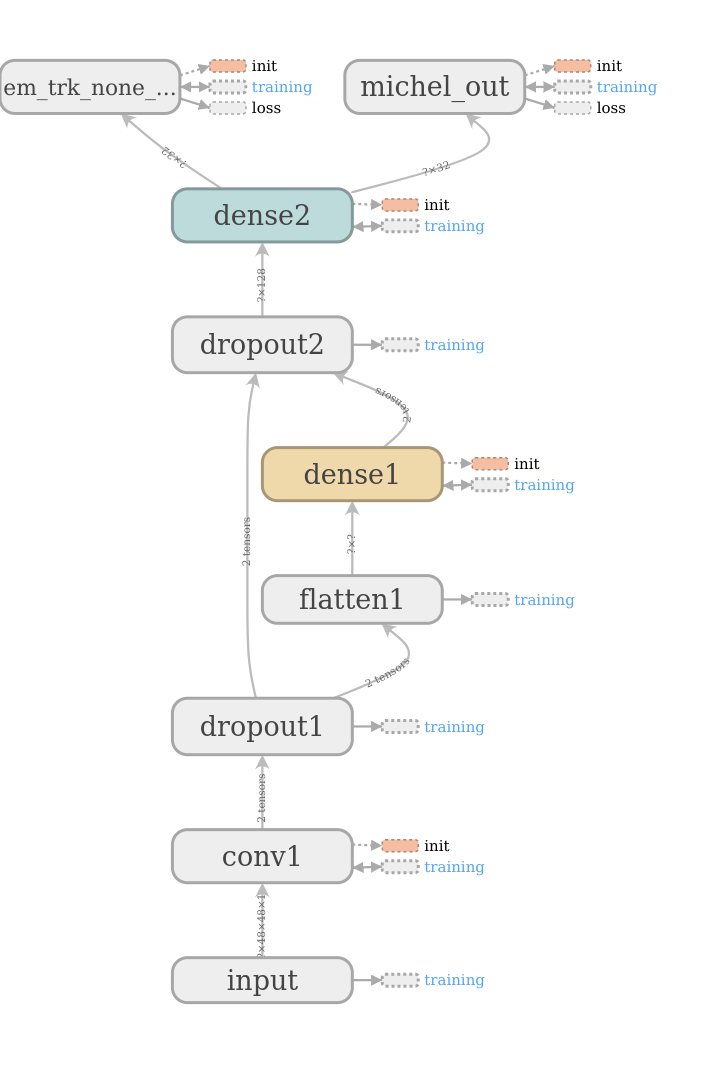
\includegraphics[width=0.6\textwidth]{figures/network_graph.png}
	\caption[Network architecture used for hit classification.]{Network
	architecture used for hit classification, visualisation from the TensorBoard
	library.}
	\label{fig:arch}
\end{figure}

The network was trained using stochastic gradient descent (SGD) with the total
loss being the weighted sum of the losses for the two output branches, \(L_{tot}
= 0.1 \cdot L_{tse} + L_m\), where the Michel classifier is given higher
precedence due to the smaller training data set available for the Michel output.
In order to speed up the learning process and converge on an optimal model, both
the momentum and decay algorithms were used; momentum reduces oscillations of
the weights during learning, while the decay of the learning rate allows for
rapid learning during early stages of SGD and increased precision as the model
converges \cite{Reed:1998:NSS:552600}. Learning metrics were monitored during
training using TensorBoard. The losses for each branch as well as the total loss
for the validation data set are given in figure \ref{fig:training} as a function
of the training epoch. The validation losses remain stable giving an indication
that regularisation with dropout was successful in preventing over--fitting of
the training data. However, the validation set loss does not increase
significantly after the first couple of epochs and so the training could have
been terminated sooner with this network architecture. The final losses measured
with the test data set are given in table \ref{tab:losses}. 

\begin{figure}[h]
	\centering
	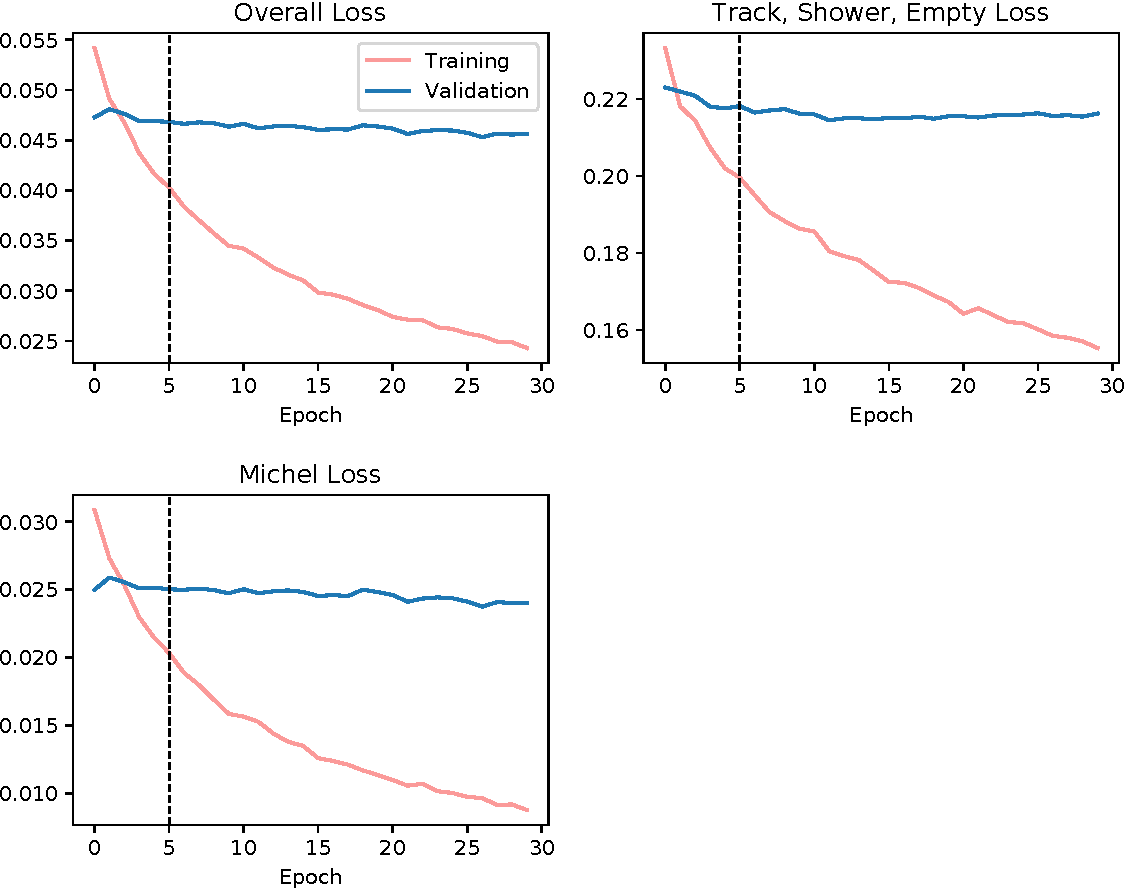
\includegraphics[width=\textwidth]{figures/losses_prelu.pdf}
	\caption[Validation and training set losses.]{Evolution of the validation
	and 
	training set losses during the training process.}
	\label{fig:training}
\end{figure}

\begin{table}[h]
	\centering
	\begin{tabular}{c|c|c|c}
		Loss Type   & \(L_{tot}\) & \(L_{tse}\) & \(L_m\) \\ \hline
		Loss Value  & 0.033       & 0.155       & 0.017   \\
	\end{tabular}
	\caption[Test set losses.]{Test set losses after full training process.}
	\label{tab:losses}
\end{table}

\section{Performance on ProtoDUNE--SP Simulation} \label{cnn-perf-sim}

The performance of the hit tagging was evaluated with reconstructed events in
the ProtoDUNE--SP detector from the latest simulation samples; in the
simulations, the detector was simulated under a number of different conditions,
specifically including the space charge effect (SCE) \cite{Mooney:2015kke} and
excluding it. The hit tagging was trained on a part of the simulated data set
which included the SCE and, as such, the samples without the SCE can be used as
a validation that the network is robust to SCE differences between the
simulations, and hence between the simulations and the data.

The distributions of the shower like classifier output for true shower hits and
all other hits are given in figure \ref{fig:show_output}; a strong separation
between track and shower hits is observed. The shower classification threshold
was optimised based on the F1 metric. This metric is defined as the harmonic
mean of the precision and recall of a classifier and optimising with this score
will ensure that both precision and recall will be high in the final classifier;
for use cases where neither precision or recall is favoured, the F1 metric can
be used to optimise for the best overall performance. The value of the F1 metric
as a function of threshold is also shown in figure \ref{fig:show_output}; the
score peaks at a threshold of 0.72 with a value of 0.863 corresponding to a
precision of 0.863 and a recall of 0.863.  

\begin{figure}[h]
	\centering
	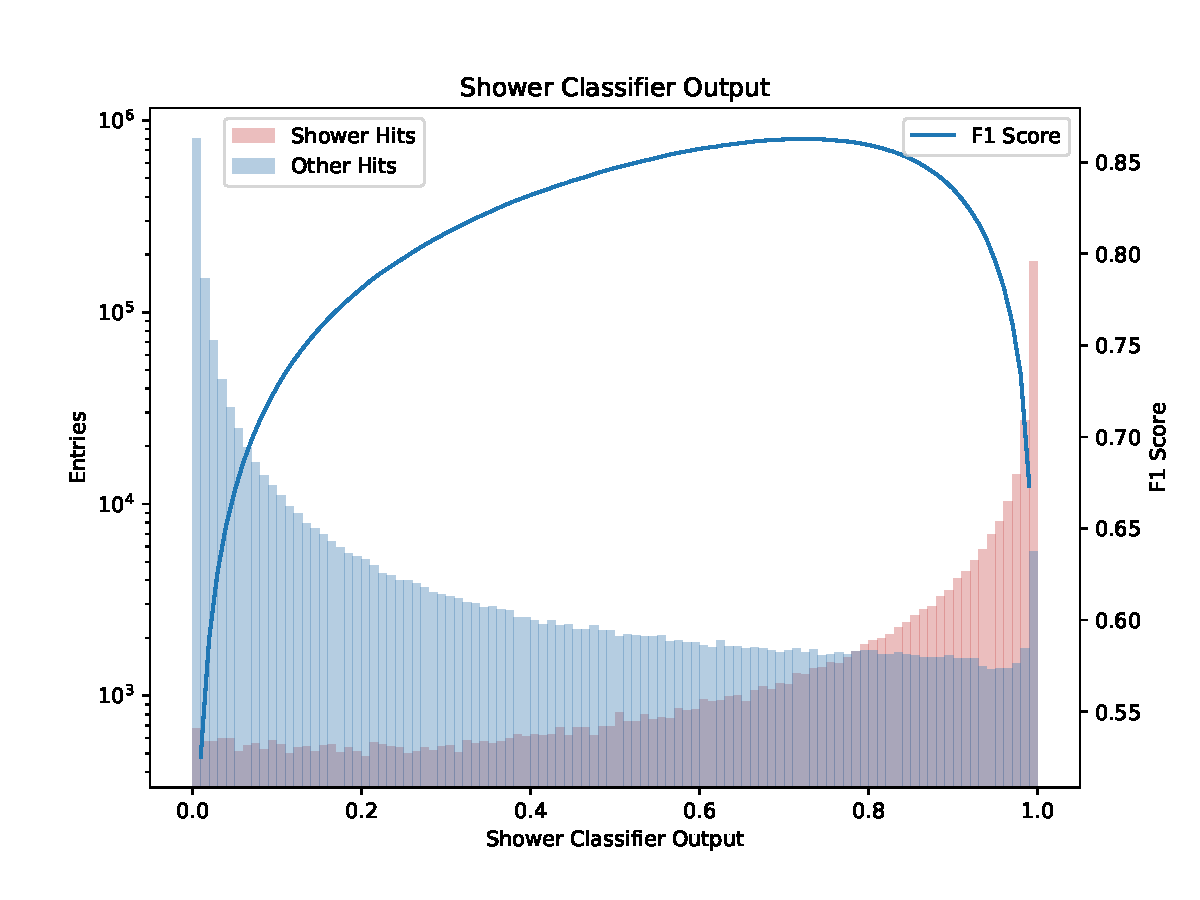
\includegraphics[width=0.8\textwidth]{figures/shower_combined.pdf} 
	\caption[Shower classifier output distributions.]{Shower classifier output
	distributions for true showers, and all other hits. Threshold optimisation
	was
	done using the F1 score metric which is also plotted.}
	\label{fig:show_output}
\end{figure}

Figure \ref{fig:michel_output} gives the distributions of the Michel classifier
output for true Michel electrons and all other hits. The large difference in
sample size between the Michel electron and other hits in this sample means that
despite high recall by the Michel electron classifier, low precision is
achieved. In chapter \ref{ch:michel} we will see that despite the low
performance of the classifier for individual hits, a pure sample of Michel
electron events can be selected by clustering hits with high Michel electron
scores. This is due to the fact that the simple hit by hit classification test
does not account for spatial correlations between Michel tagged hits.

\begin{figure}[h]
	\centering
	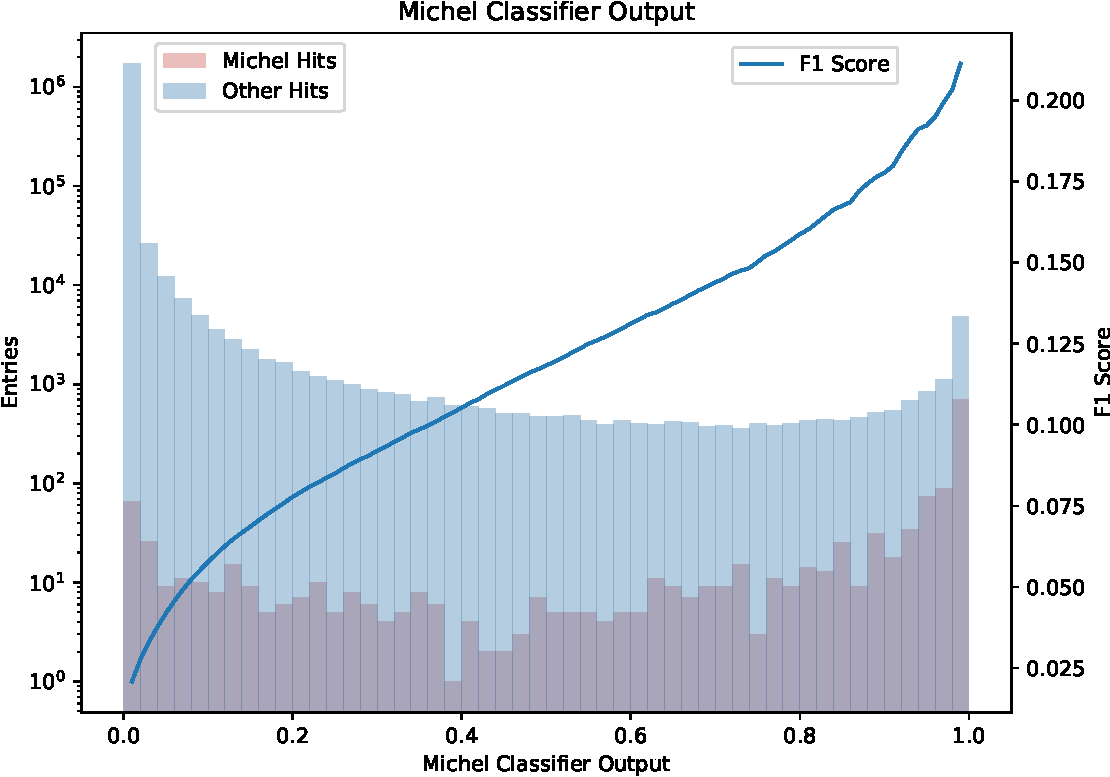
\includegraphics[width=0.8\textwidth]{figures/michel_combined.pdf} 
	\caption[Michel classifier output distributions.]{Michel classifier output
	distributions for true Michel electrons, and all other hits. Threshold
	optimisation was initially done with the F1 score metric, the threshold was
	modified when combined with a clustering algorithm, see chapter
	\ref{michel}.}
	\label{fig:michel_output}
\end{figure}

Finally, the overall performance of each classifier was evaluated using the
receiver operating characteristic (ROC) curve \cite{Fawcett2006}; ROC curves are
a test of the classification ability of a binary classifier. The curves show a
comparison of the true positive rate and the false positive rate of the
classifier as a function of the classification threshold chosen for the
classifier. Figure \ref{fig:show_roc} shows the ROC curves for the shower and
Michel classifiers; the locations of these curves in the top left corner of the
plots show that both have excellent performance as classifiers. In addition, the
ROC curves show good agreement between the SCE on and SCE off data sets, showing
that the classifiers are robust to changes in the SCE model should it differ
between data and simulation. It is worth noting that the ROC curve only accounts
for classification rates within each true sub--sample, it cannot account for the
difference in sample size between the Michel electron sample and all other hits,
and thus the ROC curve is a more instructive metric for the shower classifier
where the size of the true and false samples are of a similar magnitude.

\vspace{-5mm}

\begin{figure}[h]
	\centering
	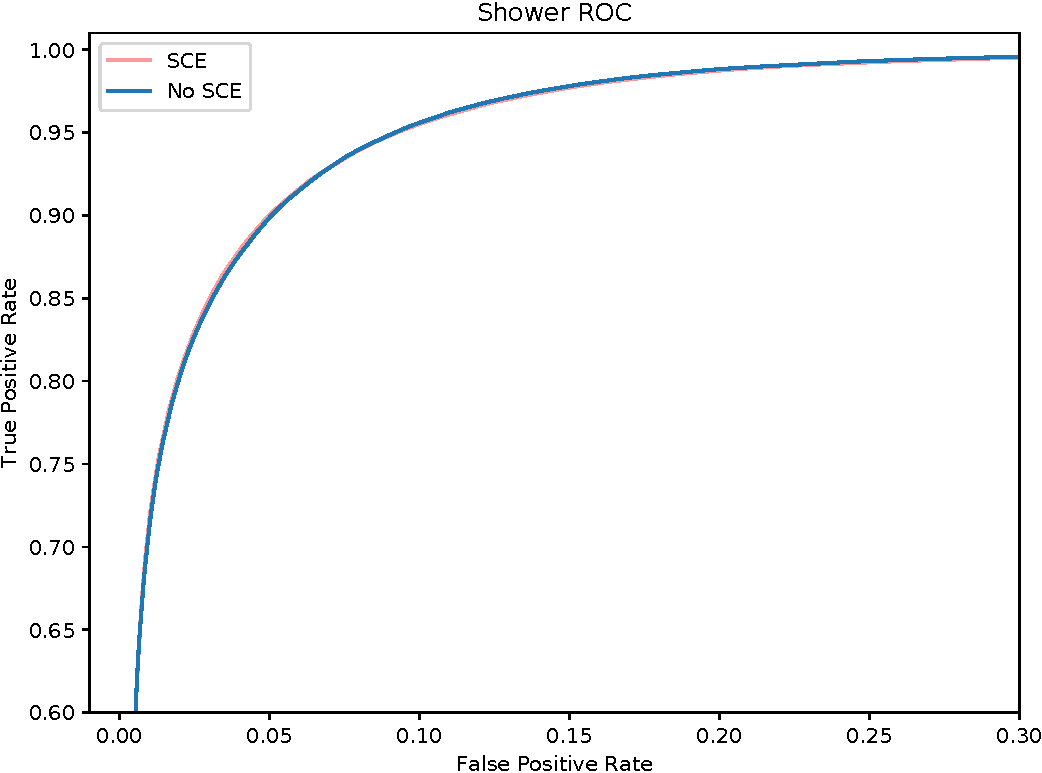
\includegraphics[width=0.65\textwidth]{figures/show_roc_comparison.pdf}
	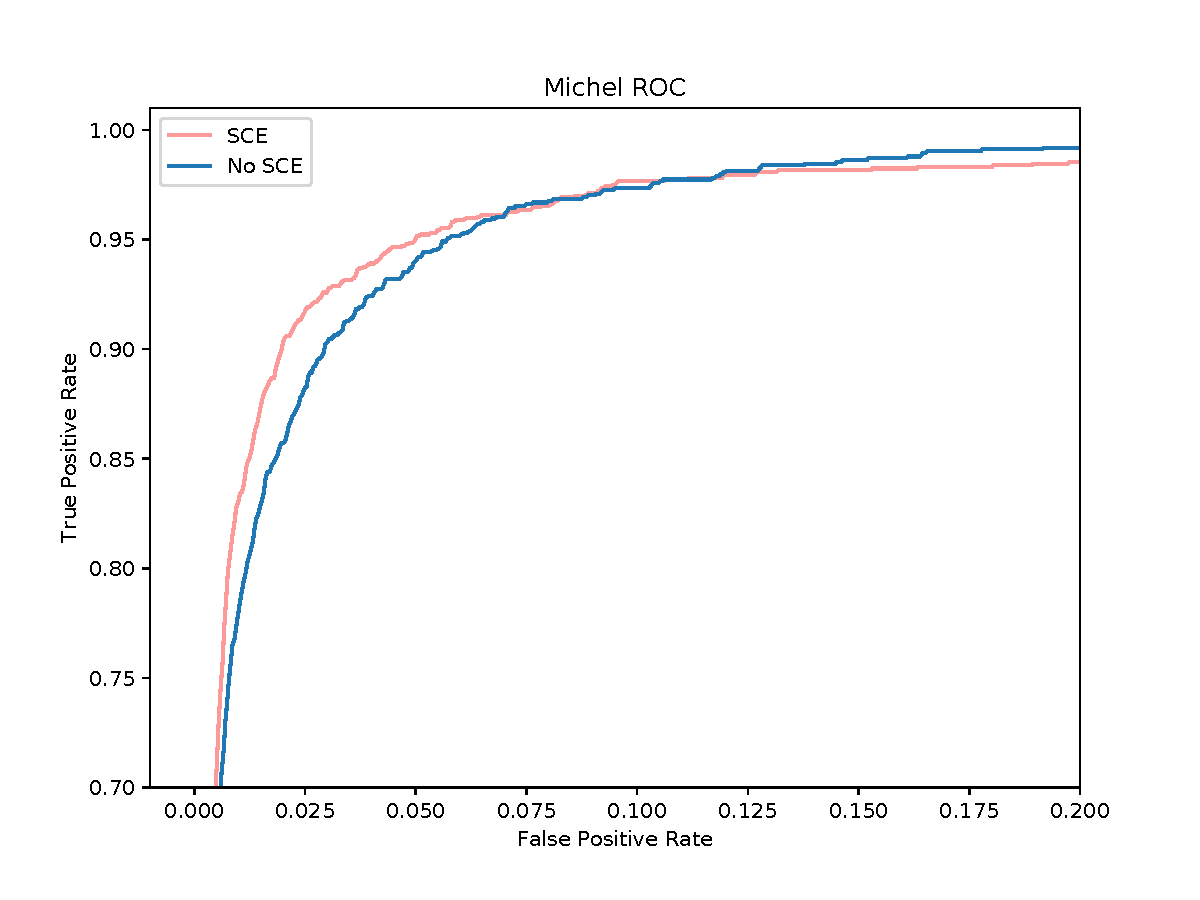
\includegraphics[width=0.65\textwidth]{figures/michel_roc_comparison.pdf}
	\caption[ROC curves.]{ROC curves for the shower (top), and Michel (bottom)
	classifiers. ROC curves for simulations including and excluding the SCE are
	included.}
	\label{fig:show_roc}
\end{figure}

\section{Validation and Performance on ProtoDUNE--SP Data} \label{cnn-perf-data}

For validation on real ProtoDUNE--SP data two approaches were used: visual
validation with event scans and cross validation with the output of the Pandora
reconstruction framework \cite{Marshall2015}. Data from ProtoDUNE--SP run number
5387 was used for the validation; the data for this run was taken under stable
operating conditions with a peak beam energy of 1 GeV. 

Hand scans of the events show qualitatively that performance on the data is
good. Figure \ref{fig:real_event} shows an example of the track like
classification of hits in a real event. We can see that for hits along the
tracks the classifier produces a large output score, and for shower like
activity in the event the score is low, as we expect. In particular the
classifier is able to identify that hits which are adjacent to the track, delta
rays, are from scattered electrons.

\begin{figure}[h]
	\centering
	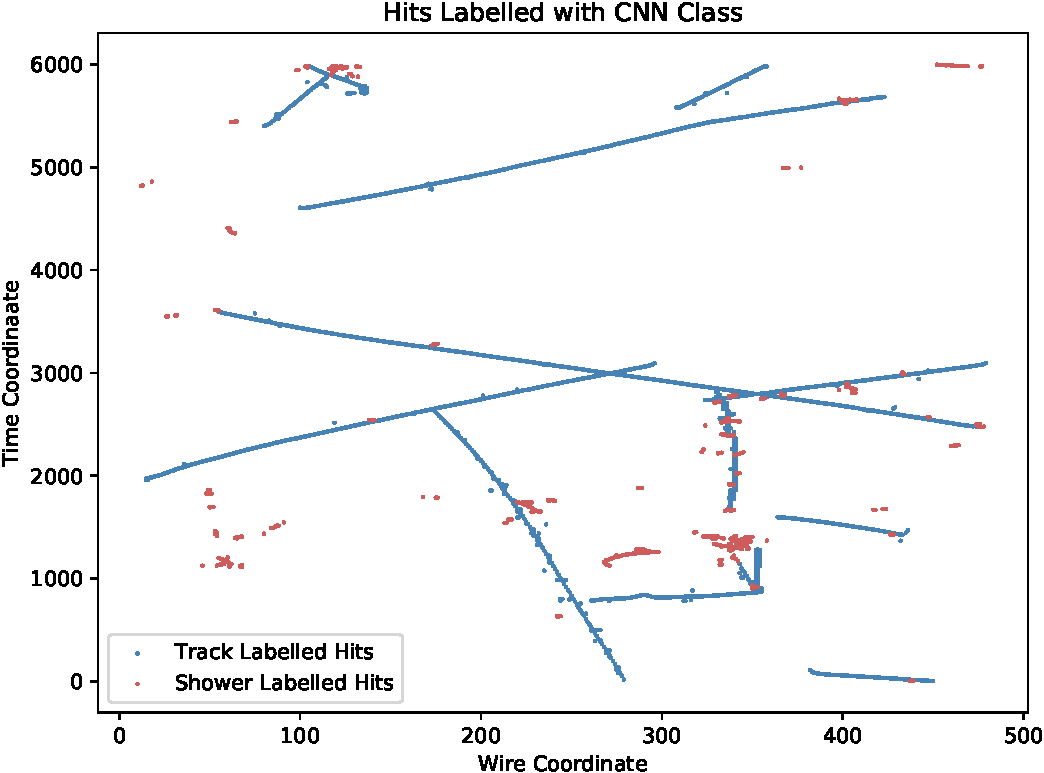
\includegraphics[height=0.45\textheight]{figures/track_score.pdf}
	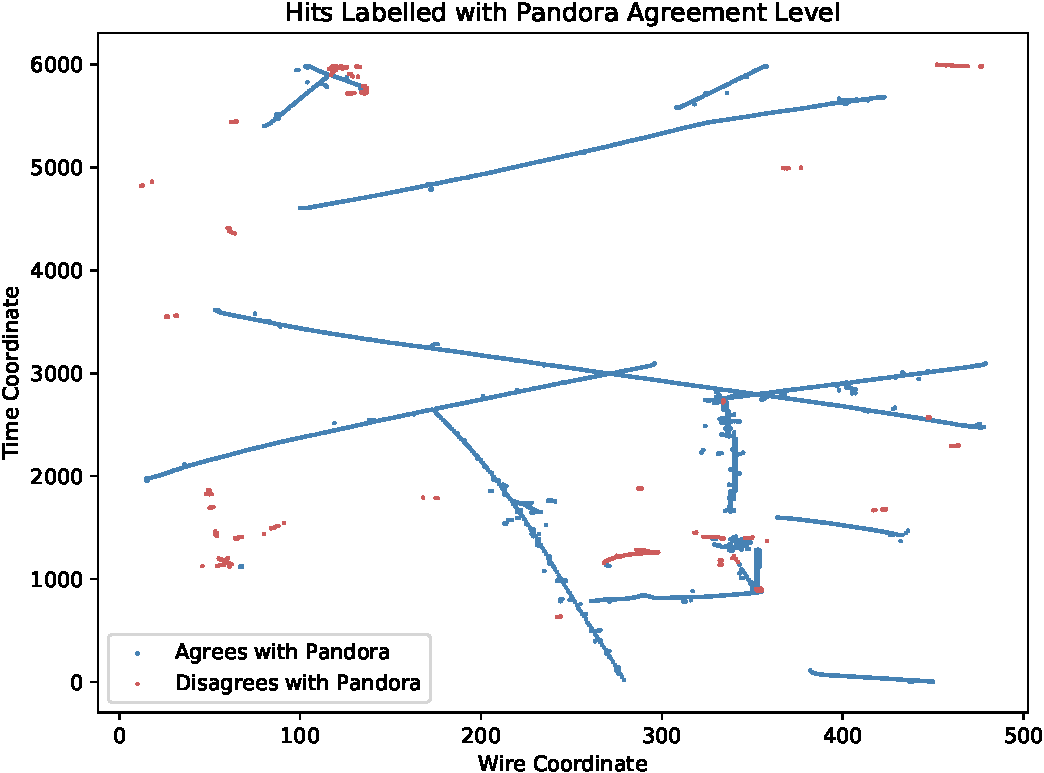
\includegraphics[height=0.45\textheight]{figures/pandora_agreement.pdf} 
	\caption[CNN output on an event from ProtoDUNE--SP data.]{Reconstructed
	hits from ProtoDUNE--SP run number 5387 labelled with CNN classification
	(top), and Pandora agreement level (bottom).}
	\label{fig:real_event}
\end{figure}

The Pandora reconstruction framework is the primary reconstruction used by the
ProtoDUNE--SP experiment; for a more quantitative validation of the performance
of the hit tagging algorithm, the hit tagging output can be compared to the
reconstructed objects produced by Pandora. After the ProtoDUNE--SP data has been
reconstructed, all of the reconstructed hits will have been clustered into
either track or shower objects. As such the comparison of a hits CNN output with
the type of reconstructed object it belongs to is a test of the agreement
between the CNN approach and the Pandora reconstruction algorithms. The Michel
electron performance cannot be validated in this way due to a lack of tagged
Michel electron objects in the Pandora output. Therefore, hand scanning of
events is the primary validation of the Michel electron classifier and will be
discussed in chapter \ref{ch:michel}.

The first test performed was the comparison of the CNN output distributions for
hits in both Pandora tracks and Pandora showers, the corresponding distributions
are given in figure \ref{fig:pandora} for both data and Monte Carlo; a strong
correlation between the reconstructed Pandora objects and the associated CNN
score can be seen in both cases, however the correlation is stronger in Monte
Carlo than in data. The discrepancy between Pandora and the CNN is still being
understood, differences between the data and simulations impact the performance
of both algorithms. Figure \ref{fig:real_event} shows reconstructed hits
labelled according to whether they agree or disagree with Pandora, we can see
that for long tracks the agreement is good while smaller objects tend to
disagree, with the CNN typically assigning a shower like classification but
Pandora reconstructing them as a track. Work to understand the discrepancy
between the CNN score and Pandora is ongoing.

\begin{figure}[h]
	\centering
	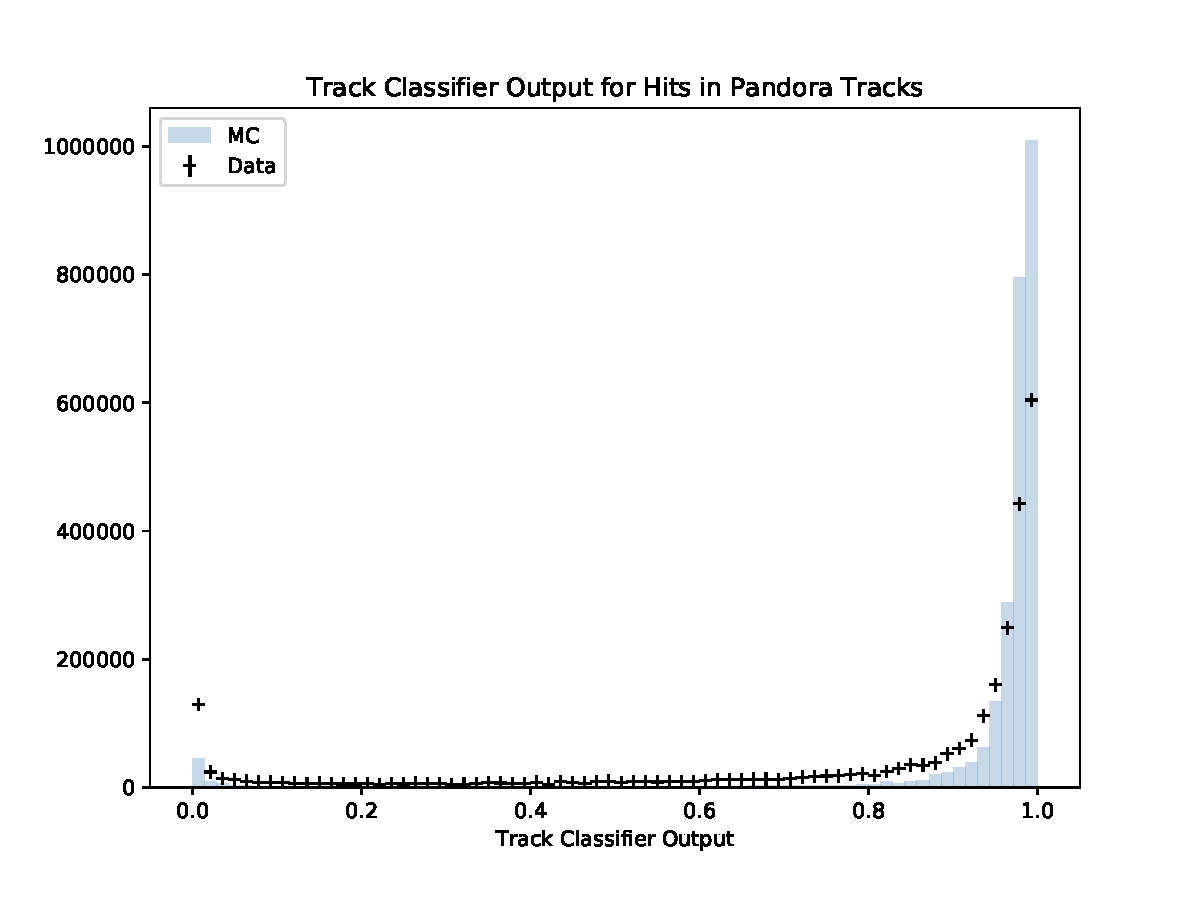
\includegraphics[width=0.7\textwidth]{figures/track_data_v_mc.pdf}
	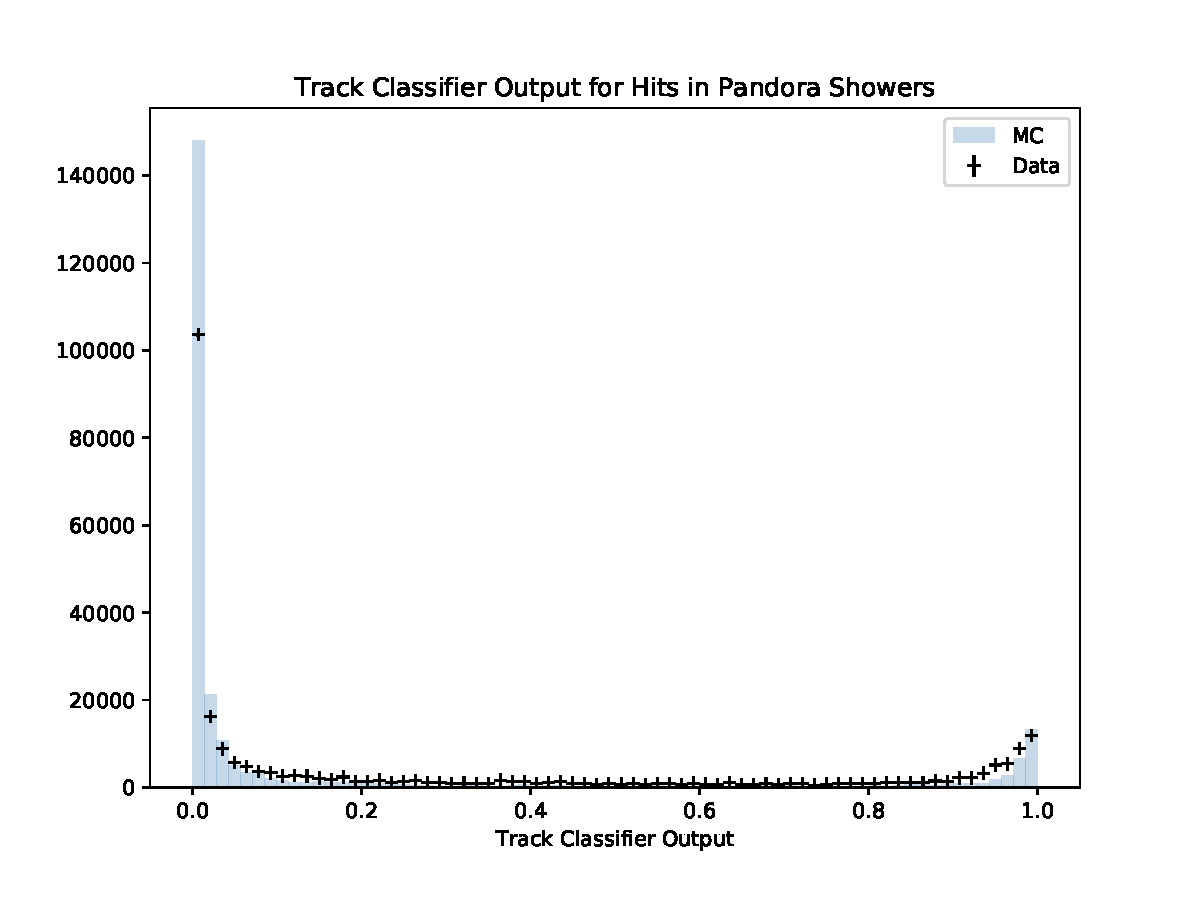
\includegraphics[width=0.7\textwidth]{figures/shower_data_v_mc.pdf}
	\caption[Output distributions for the track classifier on reconstructed
	Pandora objects.]{Output distributions for the track classifier on
	reconstructed Pandora objects.} \label{fig:pandora}
\end{figure}

This chapter has presented work on the development of a hit classification
algorithm for LArTPCs based on CNNs; the performance of this approach for
track--shower separation has been evaluated with ProtoDUNE--SP simulation and
reconstruction, demonstrating good performance. This hit tagging framework is
designed such that it can be utilised throughout the LArSoft reconstruction
chain and is complementary to other reconstruction algorithms in the framework;
chapter \ref{ch:michel} will detail an example use of the hit tagging output:
Michel electron event selection.

\noindent Additional plans for this chapter are detailed below.
\begin{itemize}[noitemsep,nolistsep]
	\item Understand the difference between data and MC when comparing the
		CNN to Pandora.
	\item Test network robustness to other detector effects in simulation. 
	\item Retrain networks with future simulations, including data
		driven models of detector effects.
\end{itemize}

